


% ============================================================================
\documentclass[11pt,letterpaper]{article}
%\usepackage[T1]{fontenc}
%\usepackage[latin1]{inputenc}
\usepackage{epic,eepic,amsmath,latexsym,amssymb,color,amsthm}
\usepackage{ifthen,graphics,epsfig,fullpage} 
\usepackage[english]{babel} 
\bibliographystyle{plain}
\usepackage{times}


% =========================================================================
\newcommand{\Xomit}[1]{}
\newcommand{\ignore}[1]{}
% =========================================================================


\begin{document}

%-----------------------for square--------------------------------------------
\newlength {\squarewidth}
\renewenvironment {square}
{
\setlength {\squarewidth} {\linewidth}
\addtolength {\squarewidth} {-12pt}
\renewcommand{\baselinestretch}{0.75} \footnotesize
\begin {center}
\begin {tabular} {|c|} \hline
\begin {minipage} {\squarewidth}
\medskip
}{
\end {minipage}
\\ \hline
\end{tabular}
\end{center}
}  
 
%--------------------------------------------------------------------
%--------------------------------------------------------------------
%-------- macros for algorithm ---------------------------------------
\newtheorem{definition}{Definition}
\newtheorem{theorem}{Theorem}
\newtheorem{lemma}{Lemma}
\newtheorem{corollary}{Corollary}
\newcommand{\toto}{xxx}
\newenvironment{proofT}{\noindent{\bf
Proof }} {\hspace*{\fill}$\Box_{Theorem~\ref{\toto}}$\par\vspace{3mm}}
\newenvironment{proofL}{\noindent{\bf
Proof }} {\hspace*{\fill}$\Box_{Lemma~\ref{\toto}}$\par\vspace{3mm}}
\newenvironment{proofC}{\noindent{\bf
Proof }} {\hspace*{\fill}$\Box_{Corollary~\ref{\toto}}$\par\vspace{3mm}}


\newcounter{linecounter}
\newcommand{\linenumbering}{\ifthenelse{\value{linecounter}<10}
{(0\arabic{linecounter})}{(\arabic{linecounter})}}
\renewcommand{\line}[1]{\refstepcounter{linecounter}\label{#1}\linenumbering}
\newcommand{\resetline}[1]{\setcounter{linecounter}{0}#1}
\renewcommand{\thelinecounter}{\ifnum \value{linecounter} > 
9\else 0\fi \arabic{linecounter}}

%----------------------------------------------------------------------

\title{\bf STM systems: Enforcing strong isolation\\
           between transactions and non-transactional code}

\author{Tyler Crain$^{\dag}$
~~~~~~~Eleni Kanellou$^{\dag}$
~~~~~~~Michel  Raynal$^{\star,\dag}$
\\~\\
$^{\star}$Institut Universitaire de France\\
$^{\dag}$IRISA, Universit\'e de Rennes 35042 Rennes Cedex, France \\
{\small {\tt \{tyler.crain, eleni.kanellou, michel.raynal\}@irisa.fr}}
}

\date{}

\maketitle


\begin{abstract}
The aim of a transactional memory system is to discharge  
programmers from the explicit  management of synchronization issues. 
To that end it suplies them with the concept of an atomic execution unit 
called  {\it transaction}. The programmer has then to  state 
only which parts of her multiprocess program have to be executed atomically. 
But, there are  applications in which shared data are 
atomically  accessed by both  transactions and non-transactional code. 
To overcome the associated consistency problems, a transactional 
memory system must provide  {\it strong isolation}. Strong isolation 
enforces ordering between transactions and conventional 
read or write operations and preserves transaction atomicity even with 
respect to non-transactional  code. 
This paper presents a transactional memory algorithm that implements 
strong isolation. This  algorithm has several interesting features: 
(a)  concurrency control of non-transactional operations is not based 
on locks and is particularly efficient and (b) any non-transactional
read or write operation always terminates (there no notion of commit/abort 
associated with them). 
While the proposed algorithm  is presented as an extension of TL2
(a classic well-known STM system), its principles are not restricted to
TL2  and coud  be implemented ``on top'' of other transactional memory systems.
~\\
{\bf Keywords}: Consistency, 
Non-transactional Operation,
Strong Isolation, Terminating operation, Transaction Atomicity,
Transactional Memory,  Opacity, Strong Isolation, TL2, 
Transaction Atomicity.


\end{abstract}

%==================================================================
\section{Introduction}


\paragraph{STM systems}
Transactional Memory (TM) 
\cite{herlihy93, shavit95} 
has  emerged  as  an  attempt  to allow  concurrent  programming  based  on
sequential reasoning:  
By  using  TM,  a  user  should  be able  to  write  a  correct  concurrent
application, provided she can  
create a correct  sequential program, the underlying TM  system taking
care of  the correct  implementation of  concurrency.  However,  while most
existing  TM algorithms consider applications  
where  shared  memory  will  be  accessed  solely by  code  enclosed  in  a
transaction,  it still seems   imperative to  examine the  possibility that
transactional and non-transactional code could co-exist. 



\paragraph{Strong vs weak isolation}
TM has to guarantee that transactions will be isolated from each other, but
when it  comes to transactions and non-transactional  operations, there are
two  paths a  TM system  can follow:  it may  either act  oblivious  to the
concurrency between transactions and non-transactional 
operations, or  it may  take this concurrency  into account and  attempt to
provid     isolation    guarantees    even   between    transactional   and
non-transactional operations. The first  case is  referred to as \emph{weak
isolation} while the second case is referred to as \emph{strong  
isolation}.  (This  distinction  of   guarantees  was  originally  made  in
\cite{blundell06},  where   reference  was  made   to  {}``weak
atomicity'' versus {}``strong atomicity''.) 

Under weak  isolation, a  TM algorithm would  be used without  much overhead
alongside  code    that  contains  non-transactional  operations.  Then,  a
non-transactional read operation  on shared  variable $x$ would  be able to
observe a write operation on $x$ which is performed by a transaction  
that has not yet committed.  Furthermore, a read operation on $x$ performed
by a  live transaction  would  be able to  observe updates on  variable $x$
that   happen   by  non-transactional   code   during  this   transaction's
execution. While this behavior  clearly violates the isolation principle of
the  transaction abstraction, it could nevertheless be anticipated and used
appropriately by the  
programmer,  still resulting  in correctly  functioning  applications. This
would require the programer 
to  be conscious  of  eventual race  conditions  between transactional  and
non-transactional code.  


\paragraph{Desirable properties}
In order  to keep consistent with  the spirit of TM  principles, however, a
system should prevent unexpected   results  from   occuring  
in presence of  race conditions. 
Furthermore, concurrency   control should  ideally be implicit  
and never be delegated to  the programmer~\cite{CIR12,MS12}.  These are the  
reasons for  which strong isolation  is desirable. Under  strong isolation,
the aforementioned scenarios,   where non-transactional operations  violate
transaction isolation, would not be allowed to happen.  

An  intuitive approach  to  achieving  strong isolation  is  to treat  each
non-transactional operation that 
accesses shared data  as a ``mini-transaction'', i.e., one  that contains a
single operation. In that case,  transactions  will have to  be  
consistent (see Section~\ref{sec:badthings})  not only with 
respect to each other, but 
also with respect to the  non-transactional operations. However, while the
concept of the memory  transaction includes the possibility of abort,
the concept of the non-transactional operation does not.  This means that a
programmer expects  that a transaction  
might fail,  either by blocking or by  aborting. Non-transactional accesses
to shared data, though,  
will usually be  read or write operations, which  the programmer expects to
be  atomic. While executing, a  read  or write  operation   is  not 
expected  to  be de-scheduled, blocked or aborted.  



\paragraph{Content of the paper}
This paper presents  a TM  algorithm which takes the
previous issues into account. This TM system is built on top of 
TL2 \cite{dice06},  a  word-based  TM algorithm  that  uses locks. 
More precisely,  TL2 is modified to accept non-transactional read 
and write operations and strong isolation in the presence of  However,  
the algorithm  is designed  without the use  of locks  for non-transactional
code, in order to guarantee that their execution will always terminate.  
To achieve  this,  apart from  offering  a modified  TL2
algorithm for transaction execution,  
the     algorithm    also     specifies     two    additional     functions,
${\sf non\_transactional\_read()}$ and ${\sf non\_transactional\_write()}$,  
which  the programmer  has to  use instead  of conventional  read  or write
operations that have to be performed  outside  of  a  transaction.  

The  possible ``bad  scenarios''  of  running
transactional and non-transactional code in  
the absence of strong isolation are reviewed in Section 
\ref{sec:badthings}. The TL2 algorithm is described in Section \ref{sec:tl2}. 
Section \ref{sec:protocol} describes  the proposed algorithm that implements
strong isolation for TL2, while  
Section \ref{sec:conclusions}  concludes the paper by  summarizing the work
and examining possible applications.  





%=======================================================================
\section{Correctness and strong isolation}
\label{sec:badthings}

\paragraph{Consistency issues}
When it comes  to environments where shared memory  is accessed exclusively
through transactions, then most accepted  
consistency   conditions    build   on   the idea of   {\it serializability}
\cite{P79}, a condition first  
established  for  the study  of  database  transactions.  For a  concurrent
execution of transactions to be serializable, it must be  
possible to find a serialization for it, i.e., a legal sequential execution
that is equivalent to it.  Serializability refers to committed  
transactions,  however. In  the  context of  memory transactions,  stricter
criteria are desirable, because even transactions that  
will  eventually abort  may cause  program  exceptions if  they observe  an
inconsistent state of the shared memory.  For this  
reason, a  prominent consistency condition for  transactional memory, which
is stricter than serializability,  has beeb proposed. 
This  consistency condition, which is called {\it opacity}
\cite{guerraoui08},  requires   that  both
committed as well as aborted transactions  
observe a  consistent state  of memory.  This implies that  in order  for a
concurrent execution of memory transactions to be  
opaque,  there must exist  an equivalent,  legal sequential  execution that
includes both committed transactions and aborted  
transactions, albeit reduced to their read prefix.

Other consistency conditions have been proposed. Among them, 
{\it virtual world consistency}~\cite{IR09} is weaker than 
opacity while keeping its spirit (i.e., it depends on both committed 
transactions and aborted transactions). 








\paragraph{Transaction vs non-transactional code}
In a  concurrent environment  shared memory  may  occasionally be
accessed by both transactions as well as  
non-transactional operations. This  is mostly brought about by  the need to
continue using legacy code that existed before  
transactional memory was  implemented. Traditionally, however, transactions
are designed to synchronize with other transactions  
and do  not take  the possibility of  non-transactional code  into account.
Traditionally, the same goes for non-transactional code: It  
is not expected from the  programmer to know the synchronization details of
the transactional memory algorithm that will run  
concurrently with  her non-transactional code.  Therefore, this possibility
of {\it co-existence of two different paradigms}, as well as  
the  fact that  transactional memory  is mostly  implemented as  a software
platform - instead of the transaction abstraction being  
directly  provided by  the hardware  -  reveal  two different  aspects that
transactional memory may acquire: In the first aspect,  
it  is  the  only way  through  which  shared  memory  may be  accessed  by
concurrent processes.  In the second aspect, which  
comes into view when it exists alongside non-transactional code, it is just
another means of achieving synchronization,  
along with  locks, fences  and other traditional 
 methods\footnote{See also the debate about whether transactions should be  
implemented through the use of locks or whether locks should be implemented
through the use of transactions.}.  

For that first aspect of transactional memory, consistency is guaranteed if
the transactional memory system implements  
opacity. For the  second aspect, however, even if  a transactional memory
system implements opacity, consistency violations  
may  still be  possible  in the  presence  of concurrent  non-transactional
code. It can be acceptable to have concurrent environments  
that may be prone to some types  of violations, as is the case with systems
that provide weak isolation \cite{blundell06, shpeis07}.  
Under weak isolation, transactional and non-transactional operations can be
concurrent. 

However, as indicated in the Introduction, transactions are considered to  
happen atomically only  with respect to other transactions.  It is possible
for non-transactional operations to see intermediate results  
of transactions that are still  live. Conversely, a transaction may see the
results of non-transactional operations that happened during  
the  transaction{}'s   execution.  If  this  behavior   is  not  considered
acceptable for an application, then the responsibility to prevent it is  
delegated   to  the   programmer  of   concurrent  applications   for  this
system. However, in order to spare the programmer this responsibility,  
both the  transactional memory algorithm  as well as  the non-transactional
read and write operations must be implemented in a way  
that  takes their co-existence  into account.  Such an  implementation that
provides synchronization  between transactional and  non-transactional code
is said to provide strong isolation.  


\paragraph{Privatization/Publication}
In  a  system  that  does  not  provide  strong  isolation,  unsynchronized
concurrent access can occur between two processes on a memory  
area that both  view as shared. However, it can also  occur on memory areas
that one of the threads views as shared while the other  
considers them to  be its private memory area. This is  referred to as the
{\it privatization problem}. An area of shared memory is privatized,  
when a process  that modified it makes it  inaccessible to other concurrent
processes\footnote{Conversely, a memory area is made public  
when it goes from being exclusively accessible by one process to being 
accessible by several processes \cite{spear08} . 
This is referred  to as the {\it publication problem} and the consistency 
issues that arise are analogous.}  \cite{spear07}.  
A typical  example of privatization would  be the manipulation  of a shared
linked list. The  removal of a node by a  transaction (for private
use   by  the process  that  invoked the  transaction) through  
non-transactional  code,  constitutes  privatization.  A  transaction  that
privatizes  a memory area   is called privatizing transaction.

Consistency problems  arise if for  example, the process that  privatized a
memory area starts accessing it non-transactionally, while the  
privatization has not become visible  to other processes, which access that
area through transactions, considering that it is still shared.  
As shown in \cite{spear07}, incorrect results due to
privatization can occur regardless of the update policy  
that a  transactional memory algorithm implements. As  an example, consider
the cases that result when given two processes $p_1$ and   
$p_2$ that privatize shared variable $x$:

\begin{itemize}
\vspace{-0.1cm}
\item  
The TM implementation  uses a  redo log.  Process $p_1$ privatizes  $x$ with
privatizing transaction $t_1$ but stalls before committing $t_1$.  
$p_2$ executes during this stall and will not see the effects of $t_1$. 
$p_2$ proceeds to privatize $x$ itself and to access it through 
non-transactional operations. The variable $x$  will still be accessed through 
transaction $t_1$ when process $p_1$ resumes and the results of $p_2$'s 
privatization will not be visible to it. 
\vspace{-0.2cm}
\item The TM implementation uses an undo log. As above, $p_2$ privatizes 
$x$ but $p_1$ stalls before performing validation before attempting 
to commit. In the meanwhile, $p_2$ executes, privatizes $x$ and commits. 
Given that updates are done in-place, $p_2$ will observe the updates 
performed by $t_1$. However, when $t_1$ resumes and attempts to commit, 
its validation will fail and it will abort. $p_2$ will be left privately 
accessing data that are no longer valid.
\end{itemize}

An STM implementation that is designed to prevent memory inconsistencies 
that may arise during privatization is called {\it privatization 
safe}. Several solutions have been proposed for the privatization problem 
such as using visible reads, conventional means of synchronization 
such as fences, sandboxing, partitioning by consensus 
\cite{scott07}, the use of lock-free 
reference   counters   \cite{afek10}  or   by  using
private transactions \cite{dice10}, to name a few. 

A system that provides {\it strong isolation} has the advantage of
inherently also solving the privatization problem. 
Strong isolation always imposes synchronization between 
transactional and non-transactional code that access memory areas that 
are potentially shared, which means that a system that guarantees strong 
isolation is inherently privatization safe.



\paragraph{Providing strong isolation}
There  are different  definitions in  literature for  strong 
isolation \cite{blundell06, harris06, maessen07}.  
In the present  paper we  will consider that strong isolation as  follows:  
\begin{enumerate}
\vspace{-0.1cm}
\item   Non-transactional   operations   are   considered   as ``mini''
transactions which never abort and  contain only a single  read or 
write operation. 
\vspace{-0.2cm}
\item The consistency condition for transactions is opacity.
\end{enumerate}
As non-transactional read an write operations never abort, 
this is called {\it terminating strong isolation} in the following.





The  first   item   implies   what   is  referred  to  as  
{\it containment}  and
{\it non-interference} \cite{blundell06}.  
Containment is   illustrated in  the  left  part of  Figure
\ref{fig:int-nonc}.  There,
under strong  isolation, we have  to assume that transaction  $T_1$ happens
atomically,  
i.e.,``all  or  nothing'',   also  with  respect  to  non-transactional
operations. Then, while $T_1$ is  alive, no non-transactional read, such as
$R_x$, should be  
able to obtain  the value written to $x$  by $T_1$. Non-interference
is  illustrated  in  the right part of Figure  \ref{fig:int-nonc}.  
Under  strong  isolation, non-transactional  
code   should  not  interfere   with  operations   that  happen   inside  a
transaction. Therefore, transaction $T_1$ should not be able to observe the
effects of  
operations $W_x$ and $W_y$, given that they happen concurrently with it. 

\begin{figure*}[h]
\centerline{
%     \mbox{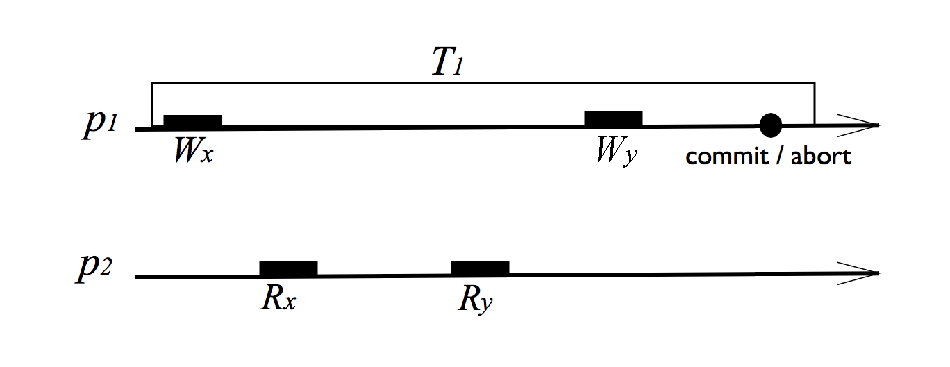
\includegraphics[width=80mm]{imgs/non_containment.eps}}
%     \mbox{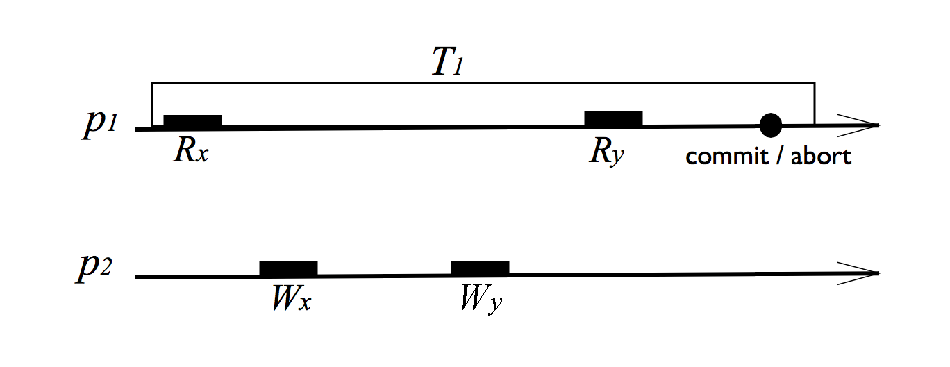
\includegraphics[width=80mm]{imgs/interference.eps}}
}
\caption{Left:  {\it Containment}  (operation $R_x$  should not  return the
    value written to $x$ inside the transaction). 
Right:  {\it  Non-Interference} (wile  it is still  executing, transaction
$T_1$ should not have access to the values that were written to $x$ and $y$
by process $p_2$).} 
\label{fig:int-nonc}
\end{figure*}


Non-interference violations can be caused  by the ABA problem. Consider the
case where a transaction $T$  
pertaining  to process  $p_1$  reads variable  $x$  through read  operation
$R_x$, and finds that it contains value  
$v_1$.  Before $T$  commits, and  after  $R_x$ has  completed, assume  that
another process $p_2$ modifies $x$  
by  writing value  $v_2$ to  it through  non-transactional  write operation
$W_{1x}$. Then, assume that either the  
same process  $p_2$ or a different process  $p_3$ write non-transactionally
value $v_1$ to $x$ through operation  
$W_{2x}$. In  this case, process  $p1$ should have  a means to  detect this
occurrence and transaction $T$ should  
not commit, given that otherwise, strong isolation would be violated. 


Non-interference for  a transaction  $T_1$ can also  be compromised  by 
interaction between non-transactional  
operations  and  another  transaction   $T_2$,  as  illustrated  in  Figure
\ref{fig:timent}. There, non-transactional operation  
$R_{2x}$  reads  what transaction  $T_2$  has  written  to shared  variable
$x$. Due to maintaining consistency, it is not  
possible  to find  a  correct serialization  order where  non-transactional
operation $W_y$ does not happen during the  
duration  of transaction $T_1$,  violating non-interference.  Therefore, in
order to preserve opacity, this situation would  
have to  be detected when  transaction $T_1$ attempts to  execute operation
$R_y$ and $T_1$ would have to be aborted. 
 

\begin{figure*}[h]
\centerline{
%    \mbox{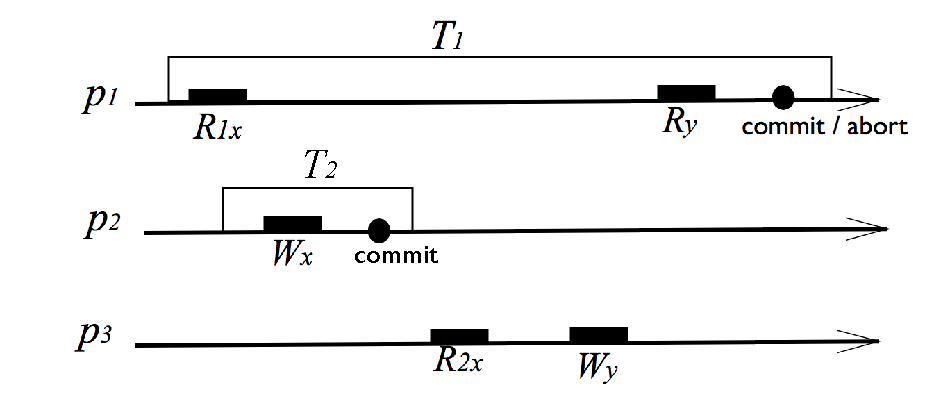
\includegraphics[width=80mm]{imgs/time_NT.eps}}
}
\caption{Transaction  $T_2$  and  non-transactional operations  of  process
$p_3$ interfere with transaction $T_1$.} 
\label{fig:timent}
\end{figure*}


\Xomit{%%%%
Many  TM algorithms,  and  so  also TL2,  already  trivially satisfy  strong
isolation and the characteristics that we consider that it implies,  
provided   that    shared   memory   is    exclusively   accessed   through
transactions. When shared memory is accessed through non-transactional  
operations also, the TM algorithm that is used has to be extended so that it
prevents the scenarios discussed above.  
} %%%\Xomit{%%%%


%========================================================================
\section{A brief presentation of TL2}
\label{sec:tl2}

This section presents the main  aspects of the  TM algorithm TL2  which  are  
used by the proposed algorithm. TL2 has been introduced by Dice, Shalev and Shavit 
in    2006    \cite{dice06}.   It does not allow for  non-transactional code.  We describe 
here the word-based version of TL2. In this  version it is considered that shared  memory 
is accessed in the granularity of  single  memory words.  For the sake of  clarity and without 
loss  of generality, the rest of the description  assumes that shared variables are the size of a 
memory word. Therefore,  the operations issued by a transaction are simply read and write operations.  



%---------------------------------------------------------------------
\subsection{Main features of TL2}
To control transaction synchronization, TL2 employs locks and 
logical dates. The variables  that a  transaction has to read form its read
set, while the variable it has to update, form its write set.  
A  transaction  first  has to  obtain  the  locks  that correspond  to  the
variables of its write set, before it can  
update them.  Conversely, a  transaction has to  check the logical dates  of the
variables in its read set, in  
order to  ensure that  the values  it has read  correspond to  a consistent
snapshot of shared memory.  


\paragraph{Locks}
TL2 locks  are stored in  a shared lock  table. Each shared memory  word is
mapped to a lock through a  
hash function\footnote{The  hash function is one-to-many,  resulting in one
lock covering several shared  
memory locations. This  partitions the memory into  so-called stripes.}. A
lock is a memory word where  
one of the  bits acts as lock  bit, indicating whether the lock  is free or
not. The rest of the bits form the  
logical date field.  The logical date of the lock  also serves as the 
logical date of the
memory  locations that  the lock  maps to.  Whenever a  shared  variable is
modified, its logical date is also updated. Due to the way the  
logical dates are assigned, they increment monotonically. 

\paragraph{Update vs read-only transactions}
TL2  makes  the  distinction  between  update  transactions  and  read-only
transactions. A {\it read-only} 
transaction consists  of a  begin phase and  an operation phase.  
An {\it update}  transaction consists  
of a  begin phase,  an operation phase,  and a  commit phase. In  an update
transaction, the operation  
phase will contain write operations to shared variables as well as possibly
read operations, while  
in a  read-only transaction, it  will solely contain read  operations. 

Read
operations in TL2 are {\it invisible},  
meaning  that when  a  transaction reads  a  shared variable,  there is  no
indication of that fact towards  
other transactions.  Write operations are  {\it deferred}, 
meaning that  TL2 does not perform the updates  
as soon as  it {}``encounters'' the shared  variables that  it has to write
to (i.e., during the operation  
phase). Instead, the updates it has to perform are logged into a local list
(also called  redo log) and   are  applied  to the shared  memory only once
the transaction is certain  to commit (i.e. which occurs  during the
commit phase). 


\paragraph{Logical time}
In order to implement logical time, TL2 employs an integer logical 
clock denoted  
$\mathit{GVC}$. Th? $\mathit{GVC}$ is incremented by update 
transactions when they attempt to commit. When it starts up, 
a transaction reads the current value of 
the $\mathit{GVC}$ into a local variable called $\mathit{rv}$. When a 
transaction attempts to commit, it performs an increment-and-fetch on 
$\mathit{GVC}$, and stores the 
return value in a local variable called $\mathit{wv}$
(which can be seen as a write version number  or a version timestamp). 
Should the transaction commit, it will write its $\mathit{wv}$ in the 
logical date field 
of all shared variables in its write set. 

Timestamping with logical dates facilitates read set validation for a 
transaction. 
When the read set of a transaction is 
not valid,  the transaction  cannot commit. The  read set of  a transaction
$T_A$ will be  invalidated  
if another,  concurrent transaction $T_B$ modifies shared  variable $x$ and
commits, after $T_A$  
has read $x$  but while $T_A$ is  still active. In TL2, it  can be detected
that a transaction{}'s read  
set is valid if the logical date of every  item on the read set is less 
than the
transaction{}'s $\mathit{rv}$  value. If, on the  contrary, the logical 
date of a read set  item is larger than
the $\mathit{rv}$ of the transaction,  
then this  indicates that,  in the meanwhile,  a concurrent  transaction has
performed  an   increment-and-fetch    of   $\mathit{GVC}$,   updated   the
item  and  committed,  by  writing  the  new 
$\mathit{GVC}$ value into the item{}'s  logical date field.



%========================================================================
\subsection{Inside a TL2 transaction}

\paragraph{Begin of a transaction}
When a  transaction starts  up, it  reads the current  value of  the $\mathit{GVC}$ 
and stores it into  
its local  $\mathit{rv}$ variable. A transaction  has to keep  track of the
variables in its read set and their  
versions, as well as the variables in  its write set and values that it has
to write to them. Therefore, it  
implements the  read and  write set  as local lists,  which will  be filled
during the transaction execution.  
These data structures are also initialized at start-up.

\paragraph{TL2 write}
When a transaction  has to update shared variable $x$,  it creates an entry
for it in its local write set list  
and there, it  stores $x${}'s address and the value that  has to be written
to it.  

\paragraph{TL2 read}
When  a transaction has  to read  shared variable  $x$, then,  if it  is an
update transaction, it first explores  
its local write set list in order to check whether $x$ is already contained
there. Should this be the case,  
then, in order to preserve consistency,  the value that is contained in the
write set list will be returned for  
the variable.  If the  update transaction doesn{}'t  find $x$ in  the write
set, then it proceeds as a read-only   transaction would proceed. 

Before and after reading $x${}'s value, a read-only transaction samples the
lock bit and the lock version  
corresponding to $x$. If the lock version is different before and after the
read or if the lock bit is set, then  
the transaction aborts, given that it has just detected a concurrent update
of $x$ which invalidates its read  
set.  If this  procedure, also  referred  to as  post-validation, does  not
result in aborting, then the operation can   
return the value that it has read  for $x$. If the transaction is an update
transaction, then, before returning the  
value, it  creates an entry for  $x$ in its  local read set list,  where it
stores the memory address of $x$.  

\paragraph{Attempt to commit}
After  having executed  all its  read and/or  write operations  in  the way
described before, a transaction attempts  
to commit. If  it is a read-only transaction and it  has reached this point
(i.e., has not been aborted during some  
read operation), then the post-validation that is performed after each read
has ensured that the values it has  
read for the  variables in its read set,  constitutes a consistent snapshot
of memory. Therefore, the read-only  
transaction  is considered  committed without  having to  take  any further
explicit action. 

On the contrary, an update  transaction has to explicitly verify whether it
can commit and explicitly make its  
commit  visible  to  the rest  of  transactions.  In  order to  update  the
variables in its write set, the transaction first  
has to  {}``obtain ownership'' for  them, i.e., lock  them, it then  has to
validate its read set, in order to ensure that  
by committing, it will not violate  consistency, and then it has to perform
the updates and release the locks it  
holds. 

\paragraph{Lock acquisition and $\mathit{GVC}$ increment} 
For  every item  in  the  transaction{}'s write  set,  bounded spinning  is
performed on the corresponding lock in order  
to  obtain  it.  If the  lock  acquisition  for  an  item fails,  then  the
transaction aborts. If, however, all locks are acquired  
successfully,   then  the   transaction  performs   increment-and-fetch  on
$\mathit{GVC}$ and stores the return value in  
local variable $\mathit{wv}$. This value of $\mathit{wv}$ will be stored as
the new version of the variables in the  
transaction's write set, if the transaction does not abort.

\paragraph{Validation of the read set}
In order  to determine whether the  transaction has to abort,  a final read
set validation takes place. During this  
validation, it  is verified  for all  items of the  read set  whether their
current version is still less that the transaction's  
read version, $\mathit{rv}$, as well as whether the items are not locked by
a different transaction. If it is detected  
that this is not the case  for any item, the transaction aborts. Otherwise,
the transaction can perform the intended  
updates. Read  set validation  is not necessary  in the special  case where
$\mathit{rv}$+1 = $\mathit{wv}$, given  
that this would  guarantee that no concurrent transaction  has executed and
possibly modified items of the read   set in the meanwhile.

\paragraph{Deferred updates and lock release}
The   address  and   update  value   for  each   shared  variable   in  the
transaction{}'s write set is stored in a corresponding  
entry  in the  transaction{}'s local  write set  list. Therefore,  for each
write set list entry, the update value is stored in the  
corresponding memory address. The  locks are released by atomically writing
the value of $\mathit{wv}$ to their lock  
version field  while clearing the lock bit. 




%========================================================================
\section{Implementing terminating strong  isolation}
\label{sec:protocol}

A traditional  solution to  the problem of  ensuring isolation   in the
presence of  non-transactional code consists in using  locks: Each shared
variable would then  
be associated with a lock and both transactions as well as non-transactional 
operations would have to acquire the lock before accessing the variable. In
order  to achieve strong isolation,  transactions would have to acquire the
locks of the  variables both in their read and in their write set.

Locks are already used  in TM algorithms - such as TL2  itself - where it is
however     assumed   that  shared   memory   is   only  accessed   through
transactions. The use  of locks  in a TM algorithm  entails blocking and may
even lead a process to starvation. However,  
it can be argued that  these characteristics are acceptable, given that the
programmer  accepts the fact that a  transaction has a duration and that it
may  even  fail: The  fact  that   there is  always  a  possibility that  a
transaction will abort means that the eventuality of  
failure to complete is an integral part of the transaction concept.  

On  the contrary,  when it  comes to  read or  write accesses  to  a shared
variable, a  non-transactional operation is  understood  as an
event  that  happens   atomically  and   completes.  Unfortunately   strong
isolation  implemented with  locks  entails the blocking  
of non-transactional read and write operations.

Given that this approach would be rather counter-intuitive for the 
programmer (as well as possibly detrimental for program efficiency), 
the   algorithm presented  in this  section  provides  a solution  for adding
strong isolation which does not based on locks for the execution 
of non-transactional  operations. This  algorithm builds on  the base  of TM
algorithm  TL2 and  extends it in  order to account for  non-transactional 
operations. While read   and write operations that appear inside a 
transaction follow the original TL2 algorithm rather closely (commit-time lock 
acquisition, write-back and validation of the  read set), 
the proposed algorithm 
specifies specific non-transactional read and  write operations 
that are to be used 
by the programmer, substituting conventional read and write operations. 
In the following sections, the memory setup, special data structures 
and operations will be explained.


%===================================================================
\subsection{Memory setup and data structures}


\paragraph{Memory setup}
The underlying memory system is made up of atomic read/write registers. 
Moroever some of them can also be accessed by the the following two 
operations. The operation denoted 
${\sf Fetch\&increment}()$ atomically adds one to the register and 
returns its previous value. 
 The operation denoted 
${\sf C\&S}()$ (for compare ans swap) is a conditional write. 
${\sf C\&S}(x,a,b)$ writes $b$ into $x$ iff $x=a$. In that case it 
returns $\mathit{true}$. Otherwise it returns  $\mathit{false}$. 


The proposed TL2 extension assumes that the
variables  are  of  types and  values  that  can  be   stored in  a  memory
word. This assumption aids in the clarity of the algorithm description  
but it  is also  justified by the  fact that  the algorithm extends  TL2, an
algorithm that is   designed to be word-based. 

As in TL2,  the variable $\mathit{GVC}$
acts as  global  clock  which  is incremented  by update transactions.
 Apart from a global   notion of ``time'', there exists also
a local one, and therefore, each process maintains a local  
variable denoted $\mathit{time}$,  which is used in order to keep  
track of when, with
respect to the $\mathit{GVC}$, a non-transactional operation 
or a transaction was last performed by
the  process. Each  process's  $\mathit{time}$   variable is   
therefore incremented
both through transactions and outside  
of  them. Update  transactions  increment their  $\mathit{time}$ variable  by
performing an increment-and-fetch  
on  $\mathit{GVC}$.  As  will  be explained  in  detail  later  on,
non-transactional operations update  
their $\mathit{time}$ variable either by  assigning it the value of 
the $\mathit{GVC}$, or by assigning it the  
logical date of a shared variable that they are accessing, or by incrementing
it by a factor of $\alpha$.  
In either  case, the value of $\mathit{time}$ after an update  is higher than
the value  it had before  the update\footnote{In the   following paragraphs
and algorithm listings, we will assume that the factor $\alpha$ is equal   
to $0.1$.}.

As TL2, the  algorithm maintains a  shared array of locks  and each
shared memory word  
is associated with a lock in this array. Contrary to TL2, however, a memory
word does not contain  
the value of the variable that  is stored in it. Instead, the algorithm uses
a  special memory setup:  
Each   write  operation  on   variable  $\mathit{var}$,   transactional  or
otherwise, creates an algorithm-specific data  
structure where  it stores  the value to  be written to  $\mathit{var}$, as
well as necessary meta-data.


\paragraph{T-record  and NT-record}
The  algorithm-specific  data structures  are shared  and  can be  of 
either  two  kinds, which will be referred   to as T-record and NT-record. 
A T-record is created by a transactional write operation while an 
NT-record is created by a  non-transactional write operation. A memory word
that is used to store  
variable $\mathit{var}$ will then no more contain the value of $\mathit{x}$
but will instead contain a pointer to a  
record of either of the  aforementioned types. Multiple write operations to
the variable will not  
overwrite previous values, but will instead form a list of records, as they
add the record  they created to the already existing ones. 
This  is illustrated in Figure  \ref{fig:mem_setup}. There, it is shown how
consecutive write operations on a given memory  
word $\mathit{x}$ end up forming a list  of records
which can be parsed starting  from the pointer stored in $x$. 

\begin{figure*}[h]
\centerline{
%    \mbox{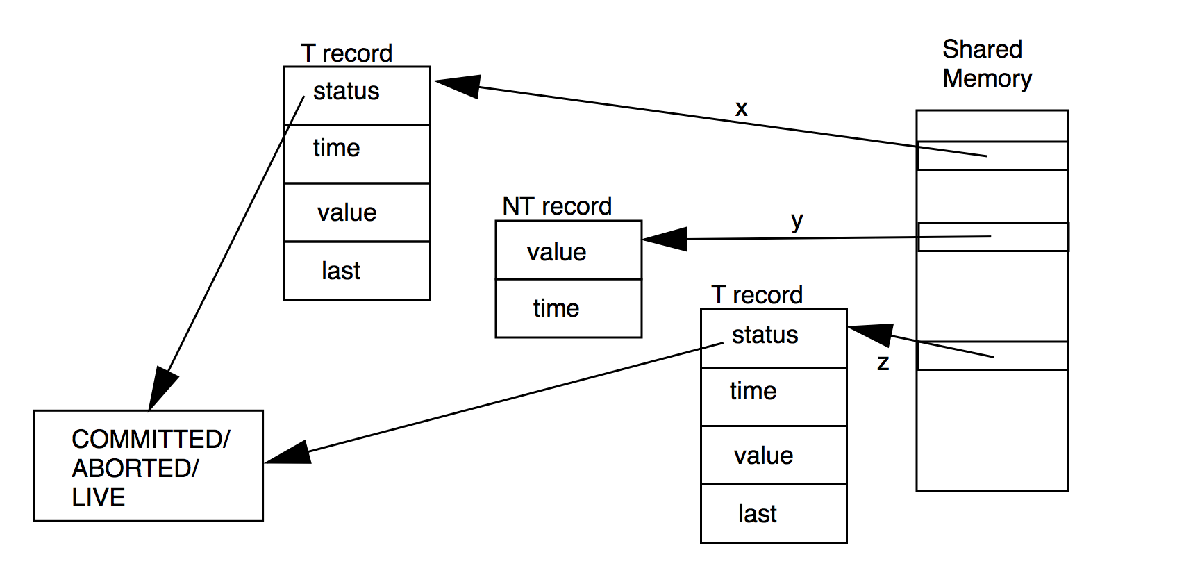
\includegraphics[width=100mm]{imgs/mem_setup_single.eps}}
}
\caption{The memory setup and the data structures that are used by the 
algorithm.}
\label{fig:mem_setup}
\end{figure*}

When  a new  T-record is  created  for variable  $\mathit{var}$ at  address
$\mathit{x}$, it is not appended  
to the list  pointed to by the pointer stored  in $\mathit{x}$. Instead, it
is placed at the head of the list.  
Contrary to that, when a  new NT-record is created, any previously existing
list is discarded  and the pointer  in $\mathit{x}$ is made to point to the
new NT-record.  

When a read operation - be it transactional or non-transactional - accesses 
a shared variable it cannot know beforehand what type of record it will find 
on the list. Therefore, it can be seen in the algorithm listings, that whenever 
a record from the list is accessed, 
the operation checks its type, i.e., it checks 
whether it is a T-record or an NT-record (for example, line \ref{A02} in Figure 
\ref{fig:ntops} contains such a check. A T-record is {}``of type T'', while an 
NT-record is {}``of type NT''). 

The  fact  that  operations  happen   concurrently  and  the  fact  that  a
transaction may  first  update a shared variable but  may then abort, makes
that the first item on the  
list  is  not   necessarily  the  current  correct  value   of  the  shared
variable. Faced with a  variable  representation that consists of a list of
records, a read operation,  
transactional or otherwise, needs to determine which record in the list is the 
relevant one.  This is done by  evaluating the meta-data of  the records in
the  list.   The  two record  types  and  the  meta-data they  include  are
described below.  


\paragraph{T-record}
A T-record is a record that consist of five fields.
\begin{itemize}
\vspace{-0.1cm}
\item[$\mathit{addr}$]
This field contains address of the memory word that is to be accessed. 
In Figure \ref{fig:mem_setup}, some records form a list which is accessed 
through the pointer stored in shared memory address $\mathit{x}$. 
Consequently, the 
value of field $\mathit{addr}$ for these records would be $\mathit{x}$.
\vspace{-0.2cm}
\item[$\mathit{status}$]
This  field  indicates  the  state  of the  transaction  that  created  the
T-record. The  
state can either be LIVE, COMMITTED or ABORTED. 
The $\mathit{status}$ field is a 
pointer to a memory location that contains information about this state.
\vspace{-0.2cm}
\item[$\mathit{time}$]
The  $\mathit{time}$  field of  a T-record  contains the  
value of  the $\mathit{GVC}$  at  the  moment the  record  was 
inserted  into the  list of   records. 
\vspace{-0.2cm}
\item[$\mathit{value}$]
This field contains the value that is meant to be written to the chosen 
memory location.
\vspace{-0.2cm}
\item[$\mathit{prev}$]
On a list of records that starts at a shared memory location, new records 
are not appended but  instead, they are placed at the head  of the list. In
order to  maintain the linking, a  pointer to the previous head of the list
is maintained. It is  represented by the field $\mathit{prev}$.
\end{itemize}

As follows from the description of  the records, the locks that are used by
this  algorithm need no longer have a logical date  field,
 given that the logical date  of a variable is stored in the $\mathit{time}$ 
field of the shared records that represent it.



\paragraph{NT-record}
Similarly to a T-record, an NT-record is also a record that consist 
of five fields:
\begin{itemize}
\vspace{-0.1cm}
\item[$\mathit{addr}$]
As for  the T-records, this field  indicates the memory  address the record
belongs  to.  In  Figure  \ref{fig:mem_setup},  this  means  that  the
NT-record pointed to by the   pointer in memory location $\mathit{y}$ would
have the value $\mathit{y}$ in its $\mathit{addr}$ field. 
\vspace{-0.2cm}
\item[$\mathit{value}$]
This field contains the value that is meant to be written to the chosen 
memory location.
\vspace{-0.2cm}
\item[$\mathit{id}$]
Each process has a unique id, denoted $\mathit{id}$. When a 
process creates an NT-record, this id is  stored in
 the  record{}'s $\mathit{id}$ field. 
This  field is used to detect cases of the ABA problem.
\vspace{-0.2cm}
\item[$\mathit{local\_time}$]
In order to avoid ABA problems, a process keeps track of multiple accesses 
that it  makes non-transactionally  to the same  memory location.  For this
operation,  the NT-record includes the field $\mathit{local\_time}$,
 which acts as an operation count by  a process on the memory location. 
\vspace{-0.2cm}
\item[$\mathit{time}$]
As in the case of T-records, the $\mathit{time}$ field of NT-records 
also stores the value 
of the $\mathit{GVC}$ at the moment the record was created. This field is 
used to avoid inconsistencies such as the ones illustrated by Figure 
\ref{fig:timent}. 
\end{itemize}

Using these control data, the most  recent valid value  of a variable  can be
determined.  Should the item at the  head of the list be of type NT-record,
then it is the most  
recent valid value  of the variable. On the other hand,  should the item at
the head of   the list be an  T-record, then if the $\mathit{status}$ field of
the record is equal to COMMITTED,  
the item represents the current valid value of the variable. Otherwise, the
first T-record  
item to  be found  with a  $\mathit{status}$ field  equal to  COMMITTED, while
traversing the list,  represents the last valid value. 



%====================================================================

\subsection{Description of the algorithm}

The main goal of the algorithm is to provide strong isolation 
in such a way that  the non-transactional  operations are never blocked. 
In order  to achieve this,  the algorithm delegates most of  
concurrency   control   and  consistency   checks   to  the   transactional
code. Non-transactional  
operations access  a memory  location without concern  about whether  it is
locked or not  and it is  up to transactions accessing the same location to
do it in a way that ensures safe  
concurrency - and to abort if this  is not possible.  As a
result, this algorithm gives high  priority   to non-transactional code. 

Given the particular memory arrangement  that the algorithm uses, two helper
procedures are used  to perform load  or store. They are
presented  in  Figure  \ref{fig:aux}\footnote{The following  notation  is
used. If $pt$ is a pointer, $pt\downarrow$ is the object pointed to by $pt$. 
if $aa$ is an object, $\uparrow aa$ is a pointer to $aa$. Hence 
$((\uparrow aa)\downarrow =aa$ and $ \uparrow(pt \downarrow)=pt$.}.


\begin{figure}[htb]
\centering{ \fbox{
\begin{minipage}[t]{150mm}
\footnotesize 
\renewcommand{\baselinestretch}{2.5} 
%\resetline
%\setcounter{linecounter}{200}
\begin{tabbing}
aaaaaaa\=aa\=aaaaa\=aa\=aa\=\kill %~\\


{\bf operation} ${\sf load}(addr)$ {\bf is}  
%\line{help1} \> 
${\sf return} (addr \downarrow)$ {\bf end operation}.  \\
\\
{\bf operation} ${\sf store}(addr, value)$ {\bf is} 
%\line{help2} \> 
$(addr \downarrow) \gets value$ {\bf end operation}.

\end{tabbing}
\normalsize
\end{minipage}
}
\caption{Helper operations for load and store operations.}
\label{fig:aux}
}
\end{figure}


In the following operation descriptions, we assume that the shared variable
that  is   accessed  by  transactional or  non-transactional operations  is
denoted $\mathit{var}$, and   
it is allocated the memory word at address $\mathit{addr}$.



%=====================================================================
\subsection{Non-transactional operations}
In  order  to  comply  with  the  algorithm a  programmer  has  to  use  the
algorithm-specific   read  and write  operations when a  variable has  to be
accessed outside of a transaction.  
Algorithms for these operations is presented in Figure \ref{fig:ntops}. 

\begin{figure}[htb]
\centering{ \fbox{
\begin{minipage}[t]{150mm}
\footnotesize 
\renewcommand{\baselinestretch}{2.5} 
%\resetline
%\setcounter{linecounter}{200}
\begin{tabbing}
aaaaaaa\=aa\=aaaaa\=aa\=aa\=\kill %~\\


{\bf operation}  ${\sf non\_transactional\_read}(\mathit{addr})$ {\bf is}\\
\line{A01} \> $\mathit{tmp} \gets {\sf load}(\mathit{addr})$; \\ 
\line{A02} \> {\bf if} $( ~\mathit{tmp}$ is of type T $ \cap \mathit{tmp.status} \neq$ COMMITTED ) {\bf then} \\
\line{A03}  \>\>  {\bf if}  $(\mathit{tmp.time}  \leq \mathit{time}  \wedge  \mathit{tmp.status} = $ LIVE) \\
\line{A04} \>\>\> {\bf then} \=${\sf \mathit{C\&S}}$($tmp.status$, LIVE, ABORTED) \\
\line{A07} \>\> {\bf end if} \\
\line{A04} \>\> {\bf if} $tmp.status = $ ABORTED {\bf then} \\
\line{A04} \>\>\> $\mathit{tmp} \gets \mathit{tmp.last}$ \\
\line{A07} \>\> {\bf end if} \\
\line{A07} \> {\bf end if} \\
\line{A10} \> $\mathit{time} \gets {\sf max}(\mathit{time}, \sf{min}(\mathit{tmp.time, GCV}))$ \\
\line{A13} \> ${\sf return}$ ($\mathit{tmp.val}$) \\
{\bf end operation}. \\
\\
{\bf operation}  ${\sf non\_transactional\_write}(\mathit{addr, value})$ {\bf is}\\
\line{B01} \> allocate new variable $\mathit{next\_write}$ of type NT; \\
\line{B03} \> $\mathit{local\_time} \gets \mathit{local\_time} + 1$; \\
\line{B04} \> $\mathit{next\_write} \gets \mathit{(addr, value, \infty, local\_time, id)}$; \\
\line{B05} \> ${\sf store}(\mathit{addr, next\_write})$ \\
\line{B02} \> $\mathit{time} \gets \mathit{GVC}$; \\
\line{B02} \> $\mathit{next\_write.time} \gets \mathit{time}$; \\
{\bf end operation}.

\end{tabbing}
\normalsize
\end{minipage}
}
\caption{Non-transactional operations for reading and writing a variable.}
\label{fig:ntops}
}
\end{figure}

\paragraph{Non-transactional read}
The   operation  ${\sf   non\_transactional\_read()}$  is   used   to  read
$\mathit{va}r$ in non-transactional code.  
The  operation first  dereferences  the pointer  stored at  $\mathit{addr}$
(line \ref{A01}). After that, the  
operation  attempts to  detect the  last valid  value of  $\mathit{var}$ by
scanning the list of records accessed  
through the pointer in $\mathit{var}$. 
If the first item of the list is a T-record that was created by a 
transaction which  has not yet  committed, it is be the  most recent
valid value and the list  
will  have to  be  traversed in  order  to find  it  (line \ref{A02},  line
\ref{A08}). Given that the list has  
a finite number of  items, the loop that is used to  scan it does terminate
(therefore it does not  
compromise the liveness requirement for the non-transactional reads). While
the operation  
traverses the  list, it detects  whether there are  items on it  which were
created by transactions that  
are still live  but that have a  $\mathit{time}$ field which is  less or equal
the process{}'s local $\mathit{time}$  
value  (line \ref{A03}).  Should  a record  with  these characteristics  be
encountered, then the transaction  
that created it has to be aborted. 
If the transaction is not aborted and the record that it created is read as 
the  most  recent valid  value  for  $\mathit{var}$,  consistency could  be
violated, given that the transaction  
could later be aborted. In this case, the non-transactional read would have
violated containment,  
which  is  why  the  algorithm  directs  the  transaction  to  be  aborted,
preemptively (line \ref{A04}).      

Once  the required  record  has been  found  and stored  in local  variable 
$\mathit{tmp}$, the local $\mathit{time}$   
variable  is updated  (lines \ref{A09}-\ref{A12}).  The updated  {\sf time}
value is used by operation  
${\sf non\_transactional\_write()}$ and is necessary in order to allow 
the detection of consistency 
violations such as the one illustrated by Figure \ref{fig:timent}. 
By advancing the value of $\mathit{time}$ 
through a non-transactional read operation, 
the serialization order of this read operation with 
respect to transactional or non-transactional operations 
that it read from is reflected. Future write 
operations by the same thread will timestamp the shared variables 
that they write to with a value  of $\mathit{time}$ greater or equal to the one 
determined by the non-transactional read, continuing to 
reflect how the operations should be correctly serialized. 

If $\mathit{tmp}$ is an NT-record, then $\mathit{time}$ is advanced to 
the maximal 
value among its current 
value and the logical date of $\mathit{tmp}$, incremented by $\alpha$ 
(taking  $0 < \alpha < 1$  entails less transactions to abort). 
If $\mathit{tmp}$ is a T-record, then $\mathit{time}$ is updated to the 
maximal value among its current value and the logical date of $\mathit{tmp}$.
 Once these book-keeping 
operations are performed, the $\mathit{value}$ field of the detected record 
is returned (line \ref{A13}).

\paragraph{Non-transactional write}
The operation ${\sf non\_transactional\_write()}$ is used to write to 
a shared variable $\mathit{var}$ 
by non-transactional code. This operation  
creates a  new  NT-record  (line  \ref{B01}),  fills  in  its  fields  (line
\ref{B04})  and 
change the pointer stored in $\mathit{addr}$ so that it references the 
new record it has created  (line \ref{B05}). 
The operation receives the address of the shared variable as well as the 
value that has to be written to it as arguments. Also in the spirit of 
providing a way to  detect consistency violations such as the one shown 
in Figure \ref{fig:timent}, the local 
variable $\mathit{time}$ is updated (line \ref{B02}).


%==================================================================
\subsection{Transactional read and write operations}

The transactional operations for performing reads and writes are 
presented in Figure \ref{fig:tops}. 

\paragraph{Transactional read}
As in TL2, when a transaction reads a shared variable, it adds it to a read
set. Differing from TL2,  
however, is  the fact that in  the present algorithm, a  transaction has to
maintain two different read sets,  
one to store T-records, called  $\mathit{rs}$, and one to store NT-records,
called $\mathit{ntrs}$. This is necessary  
because according to the type  of the record, a different validation method
will have to be used.  
The operation ${\sf  transactional\_read()}$ receives $\mathit{addr}$ as an
input argument. It starts of by checking  
whether the  desired variable already  exists in the  transaction{}'s write
set, in which  
case  the   value  stored  in  the   write  set  will   be  returned  (line
\ref{C01}). If the variable is not contained  
in  the write  set, the  pointer in  $\mathit{addr}$ is  dereferenced (line
\ref{C04}), in order to scan the list and  
determine the most recent valid value for $\mathit{var}$ 
(lines \ref{C05} - \ref{C11}). The operation preemptively 
aborts the transaction if it detects that a T-record in the 
list belongs to a not committed transaction 
while $\mathit{addr}$ is still locked (line \ref{C06}). 
The record that represents the current valid value of 
$\mathit{var}$ will be stored in local variable $\mathit{tmp}$. 

The post-validation that has to take place after a value was read is different, 
according to whether $\mathit{tmp}$ is a T-record or an NT-record. 
In case $\mathit{tmp}$ is an 
NT-record (line \ref{C12}), the post-validation consists of 
checking whether the $\mathit{time}$ 
field of the record (incremented by 0.1) is greater than the 
transaction{}'s read version number, 
stored in local variable $\mathit{rv}$ (line \ref{C15}). 
If it is, then this validation fails, and the 
transaction must abort (line \ref{C16}). However, it can occur 
that the current 
transaction is the only transaction in the system. 
Let this transaction be $\mathit{T_s}$.
Given that $\mathit{tmp}$ is an NT-record, its $\mathit{time}$ 
field was written by a non-transactional 
write operation (lines \ref{B02}, \ref{B05}). $\mathit{T_s}$ 
detects that $\mathit{tmp}$ is an NT-record, 
aborts and is then restarted.  As $\mathit{T_s}$ is assumed 
to be the only transaction in the system, 
$\mathit{GVC}$ has not been incremented by any other transaction 
between the abort of $\mathit{T_s}$ 
and its restart. This, in turn, means that the restarted 
$\mathit{T_s}$ will have the same $\mathit{rv}$ that 
it had before aborting. For this reason, when the restarted 
$\mathit{T_s}$ performs the check of line \ref{C15}, 
it will be forced to abort again. This can compromise the 
non-blocking   property   by   leading    to  an   infinite   
sequence   of  abort/restart for $\mathit{T_s}$.  
In order to avoid situations like this, $\mathit{T_s}$  performs the 
$\mathit{GVC}$ increment itself (line \ref{C16}), before ultimately aborting. 

In case $\mathit{tmp}$ is a T-record, validation is performed by checking 
whether its $ time$ field is less or 
equal to the read version number and if it is not, the transaction aborts 
(line \ref{C25}). If validation is 
successful, however, $\mathit{tmp}$ must be added to a read set. 
If $\mathit{tmp}$ is an NT-record, it will be added 
to $\mathit{ntrs}$ (line \ref{C20}), otherwise, it will be added to 
$\mathit{rs}$ (line \ref{C26}). To complete the read 
operation, the $\mathit{value}$ field of $\mathit{tmp}$ is returned 
(lines \ref{C23}, \ref{C29}).

\begin{figure} %[htb]
\centering{ \fbox{
\begin{minipage}[t]{150mm}
\footnotesize 
\renewcommand{\baselinestretch}{2.5} 
%\resetline
%\setcounter{linecounter}{200}
\begin{tabbing}
aaaaaaa\=aa\=aaaaa\=aa\=aa\=\kill %~\\


{\bf operation}  ${\sf transactional\_read}(\mathit{addr})$ {\bf is}\\
\line{C01} \> {\bf if} $\mathit{addr} \in \mathit{ws}$  {\bf then} ${\sf return}$ ($\mathit{item.value}$ from $\mathit{addr}$ in $\mathit{ws}$)  {\bf end if}; \\
\line{C04} \> $\mathit{tmp} \gets {\sf load}(\mathit{addr})$; \\
\line{C05} \> {\bf if} 
   ($\mathit{tmp}$ is of type $T \cap~ (\mathit{status} \gets \mathit{tmp.status}) \neq$ COMMITTED $)$ {\bf then} \\
\line{C06} \>\> {\bf if} $\mathit{status} =$ LIVE {\bf then} ${\sf abort}()$  {\bf else} $\mathit{tmp} \gets \mathit{tmp.last}$ {\bf end if} \\
\line{C11} \> {\bf end if}; \\
\line{C12} \> {\bf if} ($\mathit{tmp}$ is of type NT)   \\
\line{C15} \>\> {\bf then} {\bf if} $\mathit{tmp.time} >= \mathit{rv}$  \\
\> \% Do validation to prevent abort due to a non-transactional write \\
\line{C16} \>\>\> {\bf then} $\mathit{rv} \gets {\sf validate\_by\_value}()$ {\bf end if}; \\
\line{C20} \>\> {\bf if} this is an update transaction {\bf then} add $\mathit{tmp}$ to $\mathit{ntrs}$ {\bf end if}; \\
\line{C23} \>\> ${\sf return}$ $(\mathit{tmp.val})$ \\
\line{C24} \> {\bf end if}; \\
\line{C25} \> {\bf if} $(\mathit{tmp.time} > \mathit{rv})$ {\bf then} ${\sf abort}()$ {\bf end if}; \\
\line{C26} \> {\bf if} this is an update transaction 
                        {\bf then} add $\mathit{tmp}$ to $\mathit{rs}$ {\bf end if}; \\
\line{C29} \> ${\sf return}$ ($\mathit{tmp.val}$) \\
{\bf end operation}. \\
\\
{\bf operation}  ${\sf transactional\_write}(\mathit{addr, value})$ {\bf is}\\
\line{D01} \> {\bf if} $\mathit{addr} \not\in \mathit{ws}$  \\
\line{D02} \>\> {\bf then} \> allocate a new variable $item$ of type $T$; \\
\line{D03} \>\>\> $\mathit{item}  \gets (\mathit{addr, value, status, \infty})$; 
                   $\mathit{ws} \gets \mathit{ws} \cup \mathit{item}$ \\
\line{D07} \>\> {\bf else} \> set $\mathit{item.value}$ with $\mathit{addr}$ in $\mathit{ws}$ to $\mathit{value}$ \\
\line{D09} \> {\bf end if} \\
{\bf end operation}.
\end{tabbing}
\normalsize
\end{minipage}
}
\caption{Transactional operations for reading and writing a variable.}
\label{fig:tops}
}
\end{figure}

\paragraph{Transactional write}
The transactional write operations in this algorithm are performed by 
operation ${\sf transactional\_write()}$. 
It receives $\mathit{addr}$ as input value, as well as the value 
to be written to $\mathit{var}$. As  TL2, the algorithm 
performs commit-time updates of the variables it writes to. 
For this reason, the transactional write  
operation simply creates a T-record and fills in some of its 
fields (lines \ref{D02} - \ref{D03}) and also 
adds it to the transaction{}'s write set, 
if $\mathit{addr}$ was not present there (lines \ref{D01}, \ref{D03}). 
In case,  however,  the variable was already present in  the write set, the
{\sf value} field of the corresponding  
T-record is simply updated (line \ref{D07}).



\paragraph{Begin and end of a transaction} 
Book-ending a transaction are operation ${\sf begin\_transaction()}$ 
and operation ${\sf try\_to\_commit()}$, which are 
presented in Figure \ref{fig:tbc}. ${\sf begin\_transaction()}$ 
initializes local variables that will be necessary 
for the execution of the transaction, such as $\mathit{rv}$, 
$\mathit{status}$ and the read and write sets 
(lines \ref{START1}-\ref{DA2}). 

\begin{figure} [htb]
\centering{ \fbox{
\begin{minipage}[t]{150mm}
\footnotesize 
\renewcommand{\baselinestretch}{2.5} 
%\resetline
%\setcounter{linecounter}{200}
\begin{tabbing}
aaaaaaa\=aa\=aaaaa\=aa\=aa\=\kill %~\\

{\bf operation}  ${\sf begin\_transaction}()$ {\bf is}\\
\line{DA1} \> determine whether transaction is update transaction based on compiler/user input \\
\line{START1} \> $\mathit{rv} \gets \mathit{GVC}$; 
                 Allocate new variable $\mathit{status}$; \\
\line{DA2} \> $\mathit{status} \gets $LIVE; \ $\mathit{ws} \gets \emptyset$; $\mathit{rs} \gets \emptyset$; $\mathit{ntrs} \gets \emptyset$ \\
%\line{DA03} \> more??? \\
{\bf end operation}. \\
\\
{\bf operation}  ${\sf try\_to\_commit}()$ {\bf is}\\
\line{DA01} \> {\bf if} $(\mathit{ws} = \emptyset)$ {\bf then} ${\sf return}$ (COMMITTED) {\bf end if}; \\

\line{DA16} \> 
{\bf for each} $(\mathit{item} \in \mathit{ws})$ {\bf do} \\

\line{C04} \>\> $\mathit{tmp} \gets {\sf load}(\mathit{addr})$; \\


\line{C05} \>\> {\bf if} 
   ($\mathit{tmp}$ is of type $T \cap~ (\mathit{status} \gets \mathit{tmp.status}) \neq$ COMMITTED $)$ {\bf then} \\
\line{C06} \>\>\> {\bf if} $\mathit{status} =$ LIVE {\bf then} ${\sf abort}()$  {\bf else} $\mathit{item.last} \gets \mathit{tmp.last}$ {\bf end if} \\
\line{C11} \>\> {\bf else} $\mathit{item.last} \gets \mathit{tmp}$ {\bf end if}; \\


\line{DA07} \>\> {\bf if} $(\neg {\sf \mathit{C\&S}}(\mathit{item.addr, tmp, item}))$  \\
\line{DA08} \>\>\> {\bf then} $\mathit{status} \gets $ ABORTED; ${\sf abort}()$ \\
\line{DA10} \>\> {\bf end if} \\

\line{DA21} \> {\bf end for}; \\

\line{DA03} \> $\mathit{time} \gets {\sf fetch\&increment}(\mathit{GVC})$; \\

\line{DA12} \> {\bf if} $\neg{\sf validate\_all}()$  
                {\bf then} $\mathit{status} \gets $ ABORTED; ${\sf abort}()$ 
                {\bf end if}; \\


\> \% Ensure the writes haven't been overwritten by non-transactional writes \\
\line{DA16} \> 
{\bf for each} $(\mathit{item} \in \mathit{ws} \backslash \mathit{ws} \cap \mathit{rs})$ {\bf do} \\

\line{DA17} \>\> {\bf if} $(\mathit{item} \neq load(\mathit{item.addr}))$  
                 {\bf then} $\mathit{status} \gets $ ABORTED; 
                   ${\sf abort}()$ 
                {\bf end if} \\
\line{C11} \>\> $\mathit{item.time} \gets \mathit{time}$ \\
\line{DA21} \> {\bf end for}; \\
\line{DA23} \> {\bf if} ${\sf \mathit{C\&S}}$($\mathit{status}$, LIVE, COMMITTED) \\
\line{DA23'} \>\> {\bf then} \> ${\sf return}$ (COMMITTED)\\
\line{DA25} \> \> {\bf else} \= ${\sf abort}()$ \\
\line{DA26} \> {\bf end if}  \\
{\bf end operation}.

\end{tabbing}
\normalsize
\end{minipage}
}
\caption{Transaction begin/commit.}
\label{fig:tbc}
}
\end{figure}

After  performing all  required read  and write  operations,  a transaction
tries to commit, using the operation  ${\sf try\_to\_commit()}$. As in TL2,
it will be able to commit successfully, if it can acquire  
the locks for all items in its write set (line \ref{DA02}) 
and if it can validate all items in its read sets 
(lines \ref{DA12} - \ref{DA15}). However, the algorithm  differs 
here from TL2, given that 
it is faced with concurrently happening non-transactional operations. 
Non-transactional operations do not rely on locks and consequently never block. 
This, in turn, implies 
that even after acquiring the locks for all items in its write set, 
a transaction could be {}``outrun'' by 
a non-transactional operation that writes to one of those items. 
A ${\sf try\_to\_commit()}$ operation 
starts by trivially committing if the transaction was a read-only one 
(line \ref{DA01}) and by acquiring 
the locks for the write set if not. 
It then advances the $\mathit{GVC}$ (line \ref{DA03}). It is 
reminded that a ${\sf transactional\_write()}$ operation does not 
fill in the $\mathit{time}$ field of a T-record, 
because the ${\sf try\_to\_commit()}$ operation will, 
after updating the process{}'s own local variable 
$\mathit{time}$. After completing the T-record, 
the transaction attempts to place it at the head of the 
record list at $\mathit{addr}$ (lines \ref{DA04}-\ref{DA11}).
 Failure to do that implies that a non-transactional 
write operation has updated the variable, which is why the 
transaction will abort to preserve consistency. 

After having added all its write set items to the respective 
record lists for the corresponding variables 
and after having verified that its read sets are valid, the 
transaction can mark its updates as valid by 
releasing the locks of the write set items and changing its 
local $\mathit{status}$ variable from LIVE to COMMITTED.  
Before this can be done, however, it must be checked once more 
 whether the transaction{}'s updates 
have been in the meanwhile overwritten by non-transactional 
write operations. To do that, it is checked 
for each item in the write set, whether the record at the head of 
the record list at $\mathit{addr}$ is the same 
as the item. In case it is not, the transaction is aborted 
(lines \ref{DA16} - \ref{DA21}). If the transaction 
has not in the meanwhile been aborted by a non-transactional 
read operation, it will be able to 
compare-and-swap its $\mathit{status}$ variable to COMMITTED 
(lines \ref{DA22} - \ref{DA23}). In any case, 
the transaction releases the locks it holds and in case of success, 
returns COMMITTED.




\begin{figure} [htb]
\centering{ \fbox{
\begin{minipage}[t]{150mm}
\footnotesize 
\renewcommand{\baselinestretch}{2.5} 
%\resetline
%\setcounter{linecounter}{200}
\begin{tabbing}
aaaaaaa\=aa\=aaaaa\=aa\=aa\=\kill %~\\

{\bf operation} ${\sf validate\_by\_value}()$ {\bf is}\\
\line{H01} \> {\bf for each} $\mathit{item}$ in $\mathit{rs}$ {\bf do} \\
\line{H03} \>\> $\mathit{tmp} \gets load(\mathit{item.addr})$; \\
\line{H04} \>\> {\bf if} ($\mathit{tmp}$ is of type T $ \cap \mathit{tmp.status} \neq $ COMMITTED) {\bf then} \\
\line{H02} \>\>\> {\bf if} $\mathit{tmp.status} =$ LIVE $\cap \mathit{item} \not \in \mathit{ws}$
     {\bf then} ${\sf return}(\mathit{false})$ {\bf end if}; \\
\line{H05} \>\>\> $\mathit{tmp} \gets \mathit{tmp.last}$ \\
\line{H06} \>\> {\bf end if}; \\
\line{H02} \>\> {\bf if} $\mathit{item.value} \neq \mathit{tmp.value}$
     {\bf then} ${\sf return}(\mathit{false})$ {\bf end if}; \\
\line{H19} \> {\bf end for}; \\
\line{H20} \> {\bf return}$(true)$ \\
{\bf end operation}. \\
\\
{\bf operation} ${\sf abort}()$ {\bf is}\\
\line{H21} \ the transaction is aborted and restarted \\
%\line{H21} \> free items in $\mathit{ws}$, $\mathit{rs}$, and $\mathit{ntrs}$; \\
%\line{H22} \> jump to line \ref{START1} \\
{\bf end operation}. \\
\end{tabbing}
\normalsize
\end{minipage}
}
\caption{Transactional helper operations.}
\label{fig:helpers}
}
\end{figure}


\paragraph{Transactional helping operations} 
Apart from the basic operations for starting, committing, 
reading and writing, a transaction makes use of some helper 
operations that perform aborts and read 
set validations. Pseudo-code for this kind of helper operations 
is given in Figure \ref{fig:helpers}.



Operation ${\sf validate\_all()}$ is an operation that performs 
validation of both $\mathit{rs}$ and $\mathit{ntrs}$ of a transaction. 
These two read sets need different type of validation, because they 
contain different kinds of records. The 
operation returns $false$ to indicate failure and prompt the operation 
that invoked it to abort the transaction. This 
will happen if any item in $\mathit{rs}$ or $\mathit{ntrs}$ is 
locked by another transaction (line \ref{H02}, line \ref{H12}). Validation 
consists in loading the current valid item at $\mathit{addr}$ 
and storing it in local variable $\mathit{tmp}$ (lines \ref{H04}-\ref{H06}, 
lines \ref{H13} - \ref{H15}) in order to check its logical date or 
compare it to the corresponding item in the read set. 

While checking the items of $\mathit{rs}$, which will be of type 
T-record, operation ${\sf validate\_all()}$ must cause an abort, 
i.e., return $false$ in case $\mathit{tmp}$ is of type NT-record 
(line \ref{H07}) or in case $\mathit{tmp}$ is of type T-record, but the 
shared variable it corresponds to has in the meantime been updated 
by another transaction, in which case its 
logical date, reflected by the $\mathit{time}$ field of $\mathit{tmp}$, 
will be greater than the transaction{}'s read version number 
(line \ref{H08}). 

In order to validate an item of $\mathit{ntrs}$, it is checked whether 
the current valid value is a T-record, in which case 
the corresponding variable has in the meanwhile been updated by a 
different transaction, in which case the 
current transaction must again abort (line \ref{H16}). 
If, on the contrary, $\mathit{tmp}$ is of type NT-record, as it should, 
it is checked to see if, with respect to the item in the 
$\mathit{ntrs}$, it reflects an update of the corresponding shared 
variable $\mathit{var}$ by non-transactional operations of another 
process than the one that created the record 
(line \ref{H17}), or even by the process that created the record 
(line \ref{H18}). In both cases, fields of 
$\mathit{tmp}$ will not coincide with fields of the record in 
the $\mathit{ntrs}$, thereby indicating that its value is no longer valid 
and that the transaction has to be aborted.  

When a transaction is aborted in the present algorithm, 
it is immediately restarted. That is why the two operations 
provided for aborting jump to operation ${\sf begin\_transaction()}$.
 Operation ${\sf abort()}$ frees the memory 
allocated for write and read sets (line \ref{H21}) and then jumps to 
line \ref{START1} of ${\sf begin\_transaction()}$, 
in order to obtain a new read version number. 
Operation ${\sf abort\_keep\_ld)}$ (abort but restart with same logical date)
which is called right after 
a transactional read operation detects a failure to post-validate 
an NT-record that it has accessed, performs 
the same memory deallocations, but jumps to line \ref{START2} of  
${\sf begin\_transaction()}$, given that the 
transactional read operation that invoked it has already obtained 
a new read version number (line \ref{C16}).



%========================================================================

\section{Conclusion}
\label{sec:conclusions}
This paper has presented an algorithm that achieves non-blocking strong 
isolation  ``on top of'' a TM algorithm based on logical dates and locks, 
namely  TL2. 
In case of conflict of a transactional and a non-transactional
operation on a shared variable, this algorithm gives priority to 
the non-transactional operation, 
reasoning that while an eventual abort or restart is part of the 
specification of the transaction,
this is not the case for conventional read or write operations. 
Due to this priority mechanism, 
the proposed algorithm is   particularly appropriate  for environments 
in which processes do not rely heavily
on the use of transactions and where non-transactional memory 
accesses are dominant. In 
such environments, strong isolation is  provided for transactions, 
while conventional read and write operations execute with a small overhead.


\Xomit{%%%%%%%%%%%%%%
In order to implement this priority mechanism, 
the algorithm will often preemptively abort transactions 
on the sole suspicion that they might violate consistency, 
even though those transactions might have 
turned out to be acceptable. This results in an algorithm that 
is not permissive, in the intuitive sense of 
permissiveness \cite{Guerraoui:2008:PTM:1432291.1432313}. 
Future work would focus on creating 
a more permissive version of the algorithm as well as on 
examining the application of some of the 
algorithm principles to non-blocking TM algorithms in order 
to equip them with mechanisms that provide strong isolation.
}  %%%%%%%%%\Xomit{%%%%%%%%%%%%%%



%========================================================================
%\bibliographystyle{unsrt}
%\bibliography{biblio}


{\small 

\begin{thebibliography}{guerraoui08}


\bibitem{afek10}
 Afek Y.,  Avni H.,   Dice D. and  Shavit N.,
Efficient lock free privatization. 
{\it Proc.  14th Int'l conference on Principles of Distributed Systems 
(OPODIS'10)}, Springer-Verlag,  LNCS , pp. 333-347, 2010. 



\bibitem{CIR12} 
Crain T., Imb D. and Raynal M., 
Towards a Universal Construction for Transaction-based Multiprocess Programs.
{\it Proc. 13th Int'l Conference on Distributed Computing and Networking
(ICDCN'12)}, 
Springer Verlag LNCS \#7129, pp. 61-75, Hong-Kong,  2012. 



\bibitem{dice10}
Dice D., Matveev A. and  Shavit N.,
 Implicit privatization using private transactions. 
{\it Proc. Workshop on transactional memory (TRANSACT'10)}, 2010.




\bibitem{dice06}
Dice D., Shalev O. and Shavit N.,
Transactional Locking II.
{\em Proc. 20th Int'l Symposium on Distributed Computing (DISC'06)},
Springer-Verlag, LNCS \#4167, pp.~194-208, 2006.


\bibitem{guerraoui08}
Guerraoui R. and  Kapalka M.,  
 On the correctness of transactional memory. 
{\it  Proc. 13th ACM SIGPLAN Symposium on Principles and Practice of 
Parallel Programming (PPoPP '08)},  ACM Press, pp.  175-184, 2008.




\bibitem{harris06}
 Harris T.,  Larus J., and  Rajwar R., 
Transactional Memory, 
{\it 2nd edition, Synthesis Lectures on Computer Architecture},  2006.




\bibitem{herlihy93}
Herlihy M.  and Moss J.M.B,
 Transactional memory: architectural support for lock-free data structures, 
{\it Proc.  of the 20th annual Int'l Symposium on Computer Architecture 
(ISCA '93)}, ACM Press, pp. 289-300, 1993. 



\bibitem{IR09} 
Imb D. and Raynal M., 
A versatile   STM protocol with invisible read operations 
that satisfies  the  virtual world consistency condition.
{\it   16th  Colloquium   on  Structural   Information   and  Communication
Complexity  (SIROCCO'09)}, 
Springer Verlag LNCS   \#5869, pp. 266-280,  2009.


\bibitem{maessen07}
 Maessen J.-W.and Arvind M.,
 Store Atomicity for Transactional Memory. 
{\it Electronic  Notes  on Theoretical  Computer Science}, 
174(9):117-137, 2007.


\bibitem{blundell06}
 Martin M.,  Blundell C.  and E. Lewis E.,
 Subtleties of Transactional Memory Atomicity Semantics. 
{\it IEEE Computer Architecture  Letters},  5(2):  2006.


\bibitem{MS12}
Matveev A. and  Shavit N.,
Towards a Fully Pessimistic STM Model. 
{\it Proc. Workshop on transactional memory (TRANSACT'12)}, 2012.



\bibitem{P79}
Papadimitriou Ch.H., 
The Serializability of Concurrent Updates. 
{\it Journal of the ACM},  26(4):631-653, 1979. 


\bibitem{scott07}
 Scott M.L.,  Spear, M.F. Dalessandro L.  and  Marathe V.J..
 Delaunay Triangulation with Transactions and Barriers. 
{\it Proc.  10th IEEE Int'l Symposium on Workload Characterization (IISWC '07)},
 IEEE Computer Society, pp. 107-113, 2007





\bibitem{shavit95}
 Shavit N. and  Touitou D.,
 Software transactional memory. 
Software Transactional Memory. 
{\it Distributed  Computing}, 10(2):99-116, 1997. 


\bibitem{shpeis07}
 Shpeisman T.,  Menon V.,  Adl-Tabatabai A.R.,  Balensiefer  S.,  Grossman D.,
 Hudson R.L., K Moore K.F.  and  Saha B., 
Enforcing isolation and ordering in STM. 
{\it ACM  SIGPLAN Noticers}, 42(6):78-88,  2007.





\bibitem{spear08}
Spear M.F.,  Dalessandro L.,  Marathe V.J. and  Scott M.L., 
Ordering-Based Semantics for Software Transactional Memory. 
{\it Proc  12th Int'l Conference on Principles of Distributed Systems 
(OPODIS '08)},  Springer-Verlag LNCS , pp. 275-294. 2008. 



\bibitem{spear07}
Spear M.F.,  Marathe V.J. Dalessandro L. and  Scott M.L., 
Privatization techniques for software transactional memory. 
{\it Proc. 26th  annual ACM symposium on Principles of Distributed Computing 
(PODC '07)}, . ACM press, pp.  338-339, 2007.



\end{thebibliography}

}

\appendix
\section{Without Changing the Memory Layout}


\begin{figure}[htb]
\centering{ \fbox{
\begin{minipage}[t]{150mm}
\footnotesize 
\renewcommand{\baselinestretch}{2.5} 
%\resetline
%\setcounter{linecounter}{200}
\begin{tabbing}
aaaaaaa\=aa\=aaaaa\=aa\=aa\=\kill %~\\


{\bf operation}  ${\sf non\_transactional\_read}(\mathit{addr})$ {\bf is}\\
\line{A01} \> $\mathit{tmp} \gets {\sf load}(\mathit{addr})$; \\ 
\line{A02} \> {\bf if} $( ~\mathit{tmp}$ is of type T $ \cap \mathit{tmp.status} \neq$ COMMITTED ) {\bf then} \\
\line{A03}  \>\>  {\bf if}  $(\mathit{tmp.time}  \leq \mathit{time}  \wedge  \mathit{tmp.status} = $ LIVE) \\
\line{A04} \>\>\> {\bf then} \=${\sf \mathit{C\&S}}$($tmp.status$, LIVE, ABORTED) \\
\line{A07} \>\> {\bf end if} \\
\line{A04} \>\> {\bf if} $tmp.status = $ ABORTED {\bf then} \\
\line{A04} \>\>\> $\mathit{tmp} \gets \mathit{tmp.last}$ \\
\line{A07} \>\> {\bf end if} \\
\line{A07} \> {\bf end if} \\
\line{A10} \> $\mathit{time} \gets {\sf max}(\mathit{time}, \sf{min}(\mathit{tmp.time, GCV}))$ \\
\line{A13} \> ${\sf return}$ ($\mathit{tmp.val}$) \\
{\bf end operation}. \\
\\
{\bf operation}  ${\sf non\_transactional\_write}(\mathit{addr, value})$ {\bf is}\\
\line{B01} \> allocate new variable $\mathit{next\_write}$ of type NT; \\
\line{B03} \> $\mathit{local\_time} \gets \mathit{local\_time} + 1$; \\
\line{B04} \> $\mathit{next\_write} \gets \mathit{(addr, value, \infty, local\_time, id)}$; \\
\line{B05} \> ${\sf store}(\mathit{addr, next\_write})$ \\
\line{B02} \> $\mathit{time} \gets \mathit{GVC}$; \\
\line{B02} \> $\mathit{next\_write.time} \gets \mathit{time}$; \\
{\bf end operation}.

\end{tabbing}
\normalsize
\end{minipage}
}
\caption{Non-transactional operations for reading and writing a variable.}
\label{fig:ntops}
}
\end{figure}






















\begin{figure} %[htb]
\centering{ \fbox{
\begin{minipage}[t]{150mm}
\footnotesize 
\renewcommand{\baselinestretch}{2.5} 
%\resetline
%\setcounter{linecounter}{200}
\begin{tabbing}
aaaaaaa\=aa\=aaaaa\=aa\=aa\=\kill %~\\


{\bf operation}  ${\sf transactional\_read}(\mathit{addr})$ {\bf is}\\
\line{C01} \> {\bf if} $\mathit{addr} \in \mathit{ws}$  {\bf then} ${\sf return}$ ($\mathit{item.value}$ from $\mathit{addr}$ in $\mathit{ws}$)  {\bf end if}; \\
\line{C04} \> $\mathit{tmp} \gets {\sf load}(\mathit{addr})$; \\
\line{C05} \> {\bf if} 
   ($\mathit{tmp}$ is of type $T \cap~ (\mathit{status} \gets \mathit{tmp.status}) \neq$ COMMITTED $)$ {\bf then} \\
\line{C06} \>\> {\bf if} $\mathit{status} =$ LIVE {\bf then} ${\sf abort}()$  {\bf else} $\mathit{tmp} \gets \mathit{tmp.last}$ {\bf end if} \\
\line{C11} \> {\bf end if}; \\
\line{C12} \> {\bf if} ($\mathit{tmp}$ is of type NT)   \\
\line{C15} \>\> {\bf then} {\bf if} $\mathit{tmp.time} >= \mathit{rv}$  \\
\> \% Do validation to prevent abort due to a non-transactional write \\
\line{C16} \>\>\> {\bf then} $\mathit{rv} \gets {\sf validate\_by\_value}()$ {\bf end if}; \\
\line{C20} \>\> {\bf if} this is an update transaction {\bf then} add $\mathit{tmp}$ to $\mathit{ntrs}$ {\bf end if}; \\
\line{C23} \>\> ${\sf return}$ $(\mathit{tmp.val})$ \\
\line{C24} \> {\bf end if}; \\
\line{C25} \> {\bf if} $(\mathit{tmp.time} > \mathit{rv})$ {\bf then} ${\sf abort}()$ {\bf end if}; \\
\line{C26} \> {\bf if} this is an update transaction 
                        {\bf then} add $\mathit{tmp}$ to $\mathit{rs}$ {\bf end if}; \\
\line{C29} \> ${\sf return}$ ($\mathit{tmp.val}$) \\
{\bf end operation}. \\
\\
{\bf operation}  ${\sf transactional\_write}(\mathit{addr, value})$ {\bf is}\\
\line{D01} \> {\bf if} $\mathit{addr} \not\in \mathit{ws}$  \\
\line{D02} \>\> {\bf then} \> allocate a new variable $item$ of type $T$; \\
\line{D03} \>\>\> $\mathit{item}  \gets (\mathit{addr, value, status, \infty})$; 
                   $\mathit{ws} \gets \mathit{ws} \cup \mathit{item}$ \\
\line{D07} \>\> {\bf else} \> set $\mathit{item.value}$ with $\mathit{addr}$ in $\mathit{ws}$ to $\mathit{value}$ \\
\line{D09} \> {\bf end if} \\
{\bf end operation}.
\end{tabbing}
\normalsize
\end{minipage}
}
\caption{Transactional operations for reading and writing a variable.}
\label{fig:tops}
}
\end{figure}









\begin{figure} [htb]
\centering{ \fbox{
\begin{minipage}[t]{150mm}
\footnotesize 
\renewcommand{\baselinestretch}{2.5} 
%\resetline
%\setcounter{linecounter}{200}
\begin{tabbing}
aaaaaaa\=aa\=aaaaa\=aa\=aa\=\kill %~\\

{\bf operation}  ${\sf begin\_transaction}()$ {\bf is}\\
\line{DA1} \> determine whether transaction is update transaction based on compiler/user input \\
\line{START1} \> $\mathit{rv} \gets \mathit{GVC}$; 
                 Allocate new variable $\mathit{status}$; \\
\line{DA2} \> $\mathit{status} \gets $LIVE; \ $\mathit{ws} \gets \emptyset$; $\mathit{rs} \gets \emptyset$; $\mathit{ntrs} \gets \emptyset$ \\
%\line{DA03} \> more??? \\
{\bf end operation}. \\
\\
{\bf operation}  ${\sf try\_to\_commit}()$ {\bf is}\\
\line{DA01} \> {\bf if} $(\mathit{ws} = \emptyset)$ {\bf then} ${\sf return}$ (COMMITTED) {\bf end if}; \\

\line{DA16} \> 
{\bf for each} $(\mathit{item} \in \mathit{ws})$ {\bf do} \\

\line{C04} \>\> $\mathit{tmp} \gets {\sf load}(\mathit{addr})$; \\


\line{C05} \>\> {\bf if} 
   ($\mathit{tmp}$ is of type $T \cap~ (\mathit{status} \gets \mathit{tmp.status}) \neq$ COMMITTED $)$ {\bf then} \\
\line{C06} \>\>\> {\bf if} $\mathit{status} =$ LIVE {\bf then} ${\sf abort}()$  {\bf else} $\mathit{item.last} \gets \mathit{tmp.last}$ {\bf end if} \\
\line{C11} \>\> {\bf else} $\mathit{item.last} \gets \mathit{tmp}$ {\bf end if}; \\


\line{DA07} \>\> {\bf if} $(\neg {\sf \mathit{C\&S}}(\mathit{item.addr, tmp, item}))$  \\
\line{DA08} \>\>\> {\bf then} $\mathit{status} \gets $ ABORTED; ${\sf abort}()$ \\
\line{DA10} \>\> {\bf end if} \\

\line{DA21} \> {\bf end for}; \\

\line{DA03} \> $\mathit{time} \gets {\sf fetch\&increment}(\mathit{GVC})$; \\

\line{DA12} \> {\bf if} $\neg{\sf validate\_all}()$  
                {\bf then} $\mathit{status} \gets $ ABORTED; ${\sf abort}()$ 
                {\bf end if}; \\


\> \% Ensure the writes haven't been overwritten by non-transactional writes \\
\line{DA16} \> 
{\bf for each} $(\mathit{item} \in \mathit{ws} \backslash \mathit{ws} \cap \mathit{rs})$ {\bf do} \\

\line{DA17} \>\> {\bf if} $(\mathit{item} \neq load(\mathit{item.addr}))$  
                 {\bf then} $\mathit{status} \gets $ ABORTED; 
                   ${\sf abort}()$ 
                {\bf end if} \\
\line{C11} \>\> $\mathit{item.time} \gets \mathit{time}$ \\
\line{DA21} \> {\bf end for}; \\
\line{DA23} \> {\bf if} ${\sf \mathit{C\&S}}$($\mathit{status}$, LIVE, COMMITTED) \\
\line{DA23'} \>\> {\bf then} \> ${\sf return}$ (COMMITTED)\\
\line{DA25} \> \> {\bf else} \= ${\sf abort}()$ \\
\line{DA26} \> {\bf end if}  \\
{\bf end operation}.

\end{tabbing}
\normalsize
\end{minipage}
}
\caption{Transaction begin/commit.}
\label{fig:tbc}
}
\end{figure}
















\begin{figure} [htb]
\centering{ \fbox{
\begin{minipage}[t]{150mm}
\footnotesize 
\renewcommand{\baselinestretch}{2.5} 
%\resetline
%\setcounter{linecounter}{200}
\begin{tabbing}
aaaaaaa\=aa\=aaaaa\=aa\=aa\=\kill %~\\

{\bf operation} ${\sf validate\_by\_value}()$ {\bf is}\\
\line{H01} \> {\bf for each} $\mathit{item}$ in $\mathit{rs}$ {\bf do} \\
\line{H03} \>\> $\mathit{tmp} \gets load(\mathit{item.addr})$; \\
\line{H04} \>\> {\bf if} ($\mathit{tmp}$ is of type T $ \cap \mathit{tmp.status} \neq $ COMMITTED) {\bf then} \\
\line{H02} \>\>\> {\bf if} $\mathit{tmp.status} =$ LIVE $\cap \mathit{item} \not \in \mathit{ws}$
     {\bf then} ${\sf return}(\mathit{false})$ {\bf end if}; \\
\line{H05} \>\>\> $\mathit{tmp} \gets \mathit{tmp.last}$ \\
\line{H06} \>\> {\bf end if}; \\
\line{H02} \>\> {\bf if} $\mathit{item.value} \neq \mathit{tmp.value}$
     {\bf then} ${\sf return}(\mathit{false})$ {\bf end if}; \\
\line{H19} \> {\bf end for}; \\
\line{H20} \> {\bf return}$(true)$ \\
{\bf end operation}. \\
\\
{\bf operation} ${\sf abort}()$ {\bf is}\\
\line{H21} \ the transaction is aborted and restarted \\
%\line{H21} \> free items in $\mathit{ws}$, $\mathit{rs}$, and $\mathit{ntrs}$; \\
%\line{H22} \> jump to line \ref{START1} \\
{\bf end operation}. \\
\end{tabbing}
\normalsize
\end{minipage}
}
\caption{Transactional helper operations.}
\label{fig:helpers}
}
\end{figure}









\end{document}
%========================================================================
 
